\documentclass[12pt,a4paper]{memoir}

% Basic setup for a handout
\usepackage[T1]{fontenc}
\usepackage{newpxtext,newpxmath}
% To enable compactitem
\usepackage{paralist}
\usepackage{tabularx}
\usepackage{nomencl} % For \nomenclature
\usepackage{makeidx} % For \index
\usepackage{ragged2e} % For \RaggedRight
\makeindex
\makenomenclature
\setsecnumdepth{subsection} % Number sections and subsections

% Allows background color to paragraphs
\usepackage[framemethod=tikz]{mdframed} 


% Rename "Chapter" to "Exercise"
\renewcommand{\chaptername}{Exercise}

% Page layout
\setlength{\textwidth}{6.5in}
\setlength{\textheight}{9in}
\setlength{\oddsidemargin}{0in}
\setlength{\evensidemargin}{0in}
\setlength{\topmargin}{0in}
\setlength{\headheight}{0.5in}
\setlength{\headsep}{0.25in}

% To embed flowcharts
\usepackage{tikz} 
  \usetikzlibrary{shapes, arrows, positioning, calc, math, arrows.meta}
% Define block styles
\tikzstyle{decision} = [diamond, draw, fill=gray, 
    text width=4.5 em, text badly centered, node distance=3 cm, inner sep = 0 pt]
\tikzstyle{whiteblock} = [rectangle, draw, node distance=2.5 cm, text width=7.2 em, text centered, rounded corners, minimum height=4 em]
\tikzstyle{widewhiteblock} = [rectangle, draw, node distance=2.5 cm, text width=4cm, text centered, rounded corners, minimum height=4 em]
\tikzstyle{blueblock} = [rectangle, draw, fill=gray!20, text width=7.2 em, text centered, rounded corners, minimum height=4 em, node distance=3 cm]  
\tikzstyle{wideblueblock} = [rectangle, draw, fill=gray!20, 
    text width=4cm, text centered, rounded corners, minimum height=4 em,
    node distance=3 cm]  
\tikzstyle{line} = [draw, -latex']
\tikzstyle{cloud} = [draw, circle, fill=red!20, node distance=3 cm,
    minimum height=2 em]


\begin{document}

% Title page
\thispagestyle{empty}
\begin{center}
    \vspace*{2in}
    {\Huge \textbf{Data analysis}} \\
    \vspace{0.5in}
    {\Large Lucas Hoogduin} \\
    \vspace{0.5in}
    {\large \today}
\end{center}
\newpage

% Table of contents (optional for handout)
\tableofcontents
\newpage

% Main content
\chapter{Sample selection}

In this exercise, you are given a population of 20 items. Your task is to select a sample of \textbf{four items} using one of the selection methods described in the subsequent sections.

\begin{table}[htbp]
\centering
\caption{Population of 20 Items}
\label{tab:population_20_items}
\begin{tabularx}{\textwidth}{@{}ccc@{}}
\toprule
\textbf{Item} & \textbf{Value} & \textbf{Random} \\
\midrule
1  & 54 & 0.621 \\
2  & 39 & 0.397 \\
3  & 77 & 0.707 \\
4  & 82 & 0.926 \\
5  & 56 & 0.758 \\
6  & 25 & 0.979 \\
7  & 46 & 0.613 \\
8  & 92 & 0.044 \\
9  & 82 & 0.336 \\
10 & 79 & 0.179 \\
11 & 23 & 0.356 \\
12 & 47 & 0.849 \\
13 & 83 & 0.853 \\
14 & 28 & 0.039 \\
15 & 97 & 0.781 \\
16 & 61 & 0.600 \\
17 & 41 & 0.772 \\
18 & 95 & 0.756 \\
19 & 68 & 0.629 \\
20 & 79 & 0.403 \\
\midrule
Total & 1254 & \\
\bottomrule
\end{tabularx}
\end{table}

\section{Simple random sampling} % (fold)
\label{sub:simple_random_sampling}

Table \ref{tab:example_pop} lists the elements in a small population that is used to explain the selection methods.

\begin{table}[htbp]
\centering
\begin{tabular*}{6 cm}{llr}
\toprule
\parbox[t]{1.5 cm}{Item no} &
\parbox[t]{2 cm}{Description} &
\parbox[t]{1 cm}{\raggedleft Value} \\

\midrule

1 & A & 700 \\
2 & B & 750 \\
3 & C & 1,000 \\
4 & D & 900 \\
5 & E & 6,000 \\
\midrule
Total & & 9,350 \\
\bottomrule

\end{tabular*}

\caption{Example sampling frame}
\label{tab:example_pop}

\end{table}
% \end{margintable}

\bigskip
In \textbf{simple random sampling}\index{simple random sampling}\index{sampling!simple random} each element in the population has the same inclusion probability. Even though the elements have different values, they play no role in the selection process. If we sample $n$ elements without replacement, the set of possible samples contains all the possible subsets of $n$ elements. For example, if we sample $n = 2$ elements from the  sampling frame in Table \ref{tab:example_pop}, the set $S$ of all possible samples contains 10 elements, as shown in Table \ref{tab:possible_srs}.

\begin{table}[htbp]
\raggedright
\begin{tabular*}{\textwidth}{@{\extracolsep{\fill}}llll}
\toprule
\parbox[t]{1.5cm}{Sample} & \parbox[t]{3.5cm}{Selected elements} &
\parbox[t]{1.5cm}{Sample} & \parbox[t]{3.5cm}{Selected elements} \\
\midrule
1 & A, B & 6 & B, D \\
2 & A, C & 7 & B, E \\
3 & A, D & 8 & C, D \\
4 & A, E & 9 & C, E \\
5 & B, C & 10 & D, E \\
\bottomrule
\end{tabular*}
\caption{Possible samples of size $n = 2$ with simple random sampling without replacement}
\label{tab:possible_srs}
\end{table}

There are ten possible samples, and each possible sample has the same probability. The sampling procedure gives each element in the population an inclusion probability greater than zero, in fact 0.40 for each element. The inclusion probability is calculated by dividing the sample size by the population size.

\begin{equation}
\text{Inclusion probability} = \frac{\text{Sample size}}{\text{Population size}}
\end{equation}

The probability mechanism used to select the sample is usually hidden when computer programs are used to select a sample. 

\bigskip
In \textbf{fixed-interval selection}\index{fixed-interval selection}\index{selection!fixed-interval}, we first calculate the \textbf{skip}\index{skip} or \textbf{sampling interval}\index{sampling interval}\nomenclature{$I$}{sampling interval} by dividing the population size $N$\nomenclature{$N$}{population size} by sample size $n$\nomenclature{$n$}{sample size}.
\begin{equation}
I = N / n
\end{equation}
We then choose a random starting point within the first interval and skip through the population with steps of $I$, selecting the elements that are hit. 

Applications of this selection method are rare for simple random sampling. A worked-out example is provided in Section \ref{sub:selection_with_probability_proportional_to_size} for selection with a probability proportional to the size, where the method is much more common.

\bigskip
For the \emph{Case: Inventories}, we choose simple random sampling to select elements from the sampling frame that contains the inventory locations at which inventory is located. The frame consisting of all empty locations is tested completely. The test is easy to carry out. Along with testing whether there are misplaced inventory items at locations that are empty according to the inventory registration, we identify empty locations that are not on the listing. This part of the procedure filters all locations that are completely in error. 

% subsection simple_random_sampling (end)

\section{Selection with probability proportional to size} % (fold)
\label{sub:selection_with_probability_proportional_to_size}

\begin{figure}[bthp]

\begin{center}

\begin{tikzpicture}[scale=0.9]
% Define the custom color
  % \definecolor{myblue}{RGB}{0,51,141}
  \definecolor{mylightgrey}{RGB}{200,200,200}

  \filldraw[fill=mylightgrey, fill opacity=0.2, draw=black] (0,0) rectangle (1.75,0.8);
  \node at (0.875, 0.4) {A};
  \filldraw[fill=mylightgrey, fill opacity=0.4, draw=black] (1.75,0) rectangle (2.5,0.8);
  \node at (2.125, 0.4) {B};
  \filldraw[fill=mylightgrey, fill opacity=0.2, draw=black] (2.5,0) rectangle (3.5,0.8);
  \node at (3, 0.4) {C};
  \filldraw[fill=mylightgrey, fill opacity=0.4, draw=black] (3.5,0) rectangle (5.75,0.8);
  \node at (4.625, 0.4) {D};
  \filldraw[fill=mylightgrey, fill opacity=0.2, draw=black] (5.75,0) rectangle (6,0.8);
  \node at (5.875, 0.4) {F};
  \filldraw[fill=mylightgrey, fill opacity=0.4, draw=black] (6,0) rectangle (8,0.8);
  \node at (7, 0.4) {G};
  \filldraw[fill=mylightgrey, fill opacity=0.2, draw=black] (8,0) rectangle (8.5,0.8);
  \node at (8.25, 0.4) {H};
  \filldraw[fill=mylightgrey, fill opacity=0.4, draw=black] (8.5,0) rectangle (10,0.8);
  \node at (9.25, 0.4) {I};
  \filldraw[fill=mylightgrey, fill opacity=0.2, draw=black] (10,0) rectangle (11.25,0.8);
  \node at (10.625, 0.4) {J};
 
\end{tikzpicture}
\caption{Visual representation of a population with ten elements and a total book value of 45. Note that element \emph{E} has a book value of 0 and therefore has an inclusion probability of 0}
\label{fig:H5_pps_selection_population}

\end{center}
\end{figure}

Figure \ref{fig:H5_pps_selection_population} shows a stylized population with ten elements and a total book value of 45. This is used to show how the selection methods in this section work. The sample size $n =$ 5. The population is summarized in Table \ref{tab:example_pop_2}. Note that the population contains element E with a value $x_E = 0$. Probability proportional to size selection methods assign zero inclusion probability to this element, in other words, there is no possibility of selecting it. When applying these methods, we should be aware of this fact. If the population contains elements with a zero book value, these elements may require special care.

\begin{table}[htbp]
\centering
\begin{tabular}{l r r}
\toprule
Element & \multicolumn{1}{c}{Value} & \multicolumn{1}{c}{Running} \\
\midrule
A & 7 & 7 \\
B & 3 & 10 \\
C & 4 & 14 \\
D & 9 & 23 \\
E & 0 & 23 \\
F & 1 & 24 \\
G & 8 & 32 \\
H & 2 & 34 \\
I & 6 & 40 \\
J & 5 & 45 \\
\midrule
Total & 45 & \\
\bottomrule
\end{tabular}
\caption{Example population}
\label{tab:example_pop_2}
\end{table}

For example, in the \emph{Case: Inventories}, we make a list of all inventory locations that have a zero book value. We then investigate if there is any inventory present at these locations.

\bigskip
The selection methods discussed in the previous subsection have in common that the inclusion probability of an element is the same for all the elements in the population. These selection methods are the only statistically valid methods for attribute sampling and CVS.

If we want to use MUS for the purpose of our audit procedure, elements in the population should be selected with a probability proportional to their size. There are advantages with regard to improved efficiency, precision, cost-effectiveness, and representativeness in using such a sampling scheme if the (audit) value of an element in the population is approximately proportional to a known auxiliary variable, such as its book value. These schemes are called \textbf{probability proportional to size}\index{probability proportional to size}.

For populations with large variations in book values, it may not be possible to select a sample that is in strict agreement with the proportionality rule. The \textbf{inclusion probability}\index{inclusion probability}\index{probability!inclusion}\nomenclature{$\pi$}{inclusion probability} of an element $i$\nomenclature{$i$}{index} with book value $x_i$\nomenclature{$x$}{book value} is given by

\begin{equation}
\pi _i = \frac{n x_i}{X}
\label{eq:inclusion_probability}
\end{equation}
where $X = \sum{x_i}$\nomenclature{$X$}{total book value of the population} denotes the total book value of the population. For all elements, it is required that these inclusion probabilities are unequal to zero, and that they cannot be larger than one ($0 < \pi_i \leq 1$). If $n > 1$ and some $x_i$ are very large, it could happen that

\begin{equation*}
\frac{n x_i}{X} > 1
\end{equation*}

For example, when we sample $n = 6$ units from the example population in Table \ref{tab:example_pop_2} with total value $X = 45$, the inclusion probability of element D with book value $x_D = 9$ is

\begin{equation*}
\frac{6 \times 9}{45} = 1.2 > 1
\end{equation*}

This is particularly true if $x_i > {X} / {n}$.
Therefore, we assign an inclusion probability $\pi_i = 1$ to these elements, That is, we ensure that they are all selected, and let $\pi_i$ be proportional to the remaining elements. Elements with inclusion probability $\pi_i = 1$ are usually referred to as \textbf{individually significant items}\index{individually significant items}, or are said to belong to the \textbf{census stratum}\index{census stratum}\index{stratum!census}.

\bigskip
When we apply a selection with a probability proportional to size, all sampling units that we select from should have the same sign to ensure consistency, mathematical accuracy, and statistical validity in the sampling process. For example, when we sample from sampling units with a positive value, negative and zero-value elements will not have a chance of selection, and the statistical conclusion will only extend to positive values. Therefore, we should pay attention to whether these elements are present in the account under review. Two distinct situations are frequently encountered when it comes to this problem. 

In the first case, negative elements are adjustments or corrections, or can be specifically assigned to the positive elements to which they pertain. The correct way to address these types of negative items is to cancel them into specific positive elements before calculating the sample size and selecting the sample. 

The second case relates to items that represent a different class of transactions so that the negative elements cannot be specifically assigned to positive elements. From an auditing perspective, this class of transactions usually has different control objectives and, as such, should be audited separately. The statistical sample is performed on the positive elements only, and the sum of all positive elements is used as an input for the calculation of the sample size.

Elements with zero values have no probability of being selected. When they are present in a population, they should be reviewed to assess for any risk. For example, in an inventory population, elements with no quantities and a certain price may not indicate issues, whereas elements with quantities but a zero price may indicate  understatement.

\bigskip
There are many selection methods with a probability proportional to size. We now discuss a few methods that are commonly used by auditors. 
% Methods with replacement are rarely used by auditors. The commonly used methods without replacement all suffer from the fact that second-order inclusion probabilities cannot be easily computed.\marginnote{See Särndal (1992) for a discussion.} 
\begin{enumerate}
\item \textit{Random monetary units.} A random sample of monetary units is selected and traced to the elements that contain them.
\item \textit{(Randomized) Fixed-interval selection.} After a random start, we take fixed intervals of \textbf{monetary units} to select elements.\footnote{This is similar to fixed-interval selection applied to \textbf{elements} in a population, see Section \ref{sub:simple_random_sampling}.}
% \item Randomized fixed-interval selection. Fixed-interval selection, where the order of the elements is randomized before the selection process, is carried out according to the \emph{fixed-interval selection} method. 
\item \textit{Cell selection.} The list of elements is divided into cells of fixed width, and a random monetary unit is selected from each cell.
\item \textit{(Modified) Sieve selection.} All elements' values larger than the opening of the sieve are selected.
% \item [Modified sieve selection] A modification of the sieve method, fixing the sample size and ensuring that all individually significant items are selected.
%\label{}
\end{enumerate}

\section{Random monetary units} \label{par:random_monetary_units}The easiest way to select elements from the population with a probability proportional to the size of the element is by first selecting $n$ random numbers between 1 and the population book value $X$, and then tracing these selected monetary units to the running total of the book values.\index{random monetary units selection}\index{selection!random monetary units}  

For example, if the 5 random numbers are 7, 43, 2, 32, and 22, then the selected elements are A, J, A, G, and D. 

The advantage of this method is that it is random. All combinations of population elements have the correct probability of constituting the sample. One disadvantage is that a population element can be selected multiple times. A further disadvantage is that individually significant items (in this example, element D has a book value greater than or equal to $X/n = 45/5 = 9$) may not be selected at all. A practical way to avoid this is to extract these elements from the population before selecting the sampling units.

\section{(Randomized) fixed-interval selection}\label{par:fixed_interval_selection} In this method, we first calculate the sampling interval 
\begin{equation}
I = X / n
\label{eq:sampling_interval}
\end{equation}
Then, a random monetary unit is selected from the first interval and every consecutive $I$th unit.\index{fixed-interval selection}\index{selection!fixed-interval}

For example, with $X =$ 45 and $n =$ 5, we calculate the interval $I = 45/5 =9$. We choose a random number between 1 and 9, in this example 2. The selected monetary units are 2, 11, 20, 29, and 38, corresponding to elements A, C, D, G, and I, respectively.

The main disadvantage of fixed-interval selection is that the number of possible samples is reduced. In this example, there are only six possible samples. This disadvantage can be overcome by randomizing the order of the sampling units in the population. This method is referred to as the \textbf{randomized fixed-interval selection}\index{randomized fixed-interval selection}\index{selection!randomized fixed-interval} 

\section{Cell selection} An improvement on the fixed-interval selection method is obtained through the \textbf{cell selection}\index{cell selection}\index{selection!cell} method. Again, we divide the total book value $X$ by the sample size $n$ to obtain cells of width $X / n = 45 / 5 = 9$, but rather than selecting the same monetary unit within each cell, we select a random one.

For example, by constructing five cells of size nine each, we obtain five random numbers, $RN = $ 0.5196, 0.0988, 0.0968, 0.7983, and 0.3822. We then indicate the selected cumulative monetary unit. Note that we do not need to round the results. In practice, we use the ceiling value for the nearest monetary value. Table \ref{tab:example_cell_selection} lists the results of these calculations.

\begin{table}[htbp]
\begin{tabular*}{11.2 cm}{lrrrc}
\toprule
\parbox[t]{1 cm}{Cell} &
\parbox[t]{1.7 cm}{\raggedleft Random number $RN$} &
\parbox[t]{2 cm}{\raggedleft Random monetary unit} &
\parbox[t]{2 cm}{\raggedleft Selected monetary unit ($\times $ 9)} &
\parbox[t]{2 cm}{Selected element} \\

\midrule

1 & 0.5196 & 0.5196 & 4.676 & A \\
2 & 0.0988 & 1.0988 & 9.889 & B \\
3 & 0.0968 & 2.0968 & 18.871 & D \\
4 & 0.7983 & 3.7983 & 34.185 & I \\
5 & 0.3822 & 4.3822 & 39.440 & I \\

\bottomrule
\end{tabular*}
\caption{Example cell selection}
\label{tab:example_cell_selection}
\end{table}

Although the disadvantages of the fixed-interval selection method now have been slightly alleviated, new problems have been introduced. First, element D, which should have a 100\% inclusion probability, may not be hit at all. This can be overcome by removing all items greater than or equal to $I$ from the population before creating the cells. Another practical problem is that elements straddling a cell boundary may be hit twice, as in the case with element I in the example. It may be counterintuitive to take the same element into account twice when evaluating the sample, and it will be difficult to explain to the client that a population cannot be approved because we found too many errors, simply because we selected an incorrect element twice.

\section{Sieve selection}

Sieve selection aims to overcome the disadvantages of previously discussed methods. This method works as follows:\index{sieve selection}\index{selection!sieve}
\begin{compactitem}
\item Calculate the sampling interval $I = X / n$.
\item For each element in the population, multiply the sampling interval $I$ with a random number $RN$\nomenclature{$RN$}{random number between 0 and 1} between 0 and 1 to obtain the sieve opening $u_i = I \times RN_i$.\nomenclature{$u$}{sieve opening}
\item Compare the book value of the $i$th element $x_i$ to the sieve opening $u_i$. If $x_i \geq u_i$, then the element is caught by the sieve and selected for testing. If $x_i < u_i$, then the element falls through the sieve and is not selected for testing.
%\label{}
\end{compactitem}

\bigskip
Applying this logic to the example population from Table \ref{tab:example_pop_2}, we obtain $I =$ 45 / 5 = 9 and the results in Table \ref{tab:example_sieve_selection}.

\begin{table}[htbp]
\begin{tabularx}{\textwidth}{%
  >{\raggedright\arraybackslash}p{1.5cm}  % Element
  >{\raggedleft\arraybackslash}p{1.5cm}   % Book value x
  X                                     % Random number RN
  X                                     % Sieve opening
  >{\centering\arraybackslash}X         % Selected?
}
\toprule
Element &
Book value $x$ &
Random number $RN$ &
Sieve opening $u = I \times RN$ &
Selected if $x \geq u$ \\
\midrule
A & 7 & 0.1465 & 1.319 & Yes \\
B & 3 & 0.9565 & 8.609 & No  \\
C & 4 & 0.0442 & 0.398 & Yes \\
D & 9 & 0.8027 & 7.224 & Yes \\
E & 0 & n/a    & n/a   & n/a \\
F & 1 & 0.4815 & 4.334 & No  \\
G & 8 & 0.7083 & 6.375 & Yes \\
H & 2 & 0.1783 & 1.605 & Yes \\
I & 6 & 0.9207 & 8.286 & No  \\
J & 5 & 0.1335 & 1.202 & Yes \\
\bottomrule
\end{tabularx}
\caption{Example sieve selection}
\label{tab:example_sieve_selection}
\end{table}

The advantages of the sieve method are that elements can be hit no more than once, and the inclusion probabilities of the elements are independent of each other. A disadvantage is that the sample size obtained is unknown in advance. We see from the results in Table \ref{tab:example_sieve_selection} that even though the desired sample size $n = $ 5, we selected six elements. This disadvantage is addressed by modifying the sieve method.

\section{Modified sieve selection} In the sieve method an element is selected if $x_i \geq I \times RN_i$. This is equivalent to $x_i / RN_i \geq I$. Instead of multiplying the sampling interval $I$ by a random number $RN_i$ and comparing it to the book value of the element, we divide the book value by a random number and compare the resulting sieve number $sn_i = x_i / RN_i$ to $I$.\nomenclature{$sn$}{sieve number} We select exactly $n$ elements with the largest sieve numbers $sn_i$.\index{modified sieve selection}\index{selection!modified sieve} 

We apply this logic to the example population and obtain the results in Table \ref{tab:example_modified_sieve_selection}. The table is sorted on descending sieve number $sn$. Note that element D is individually significant when $n = $ 5 and is automatically selected even before element H with a higher sieve number.

\begin{table}[htbp]
\begin{tabularx}{\textwidth}{lXXXX}
\toprule
Element & Book value $x$ & Random number $RN$ & Sieve number $sn = x / RN$ & Selected? \\
\midrule
C & 4 & 0.0442 & 90.50 & Yes \\
A & 7 & 0.1465 & 47.78 & Yes \\
J & 5 & 0.1335 & 37.45 & Yes \\
G & 8 & 0.7083 & 11.29 & Yes \\
H & 2 & 0.1783 & 11.22 & No \\
D & 9 & 0.8027 & 11.21 & Yes \\
I & 6 & 0.9207 & 6.52 & No \\
B & 3 & 0.9565 & 3.14 & No \\
F & 1 & 0.4815 & 2.08 & No \\
\bottomrule
\end{tabularx}
\caption{Example modified sieve selection.}
\label{tab:example_modified_sieve_selection}
\end{table}

We need to devote special attention to individually significant items: an element with a large book value may not be among the $n$ elements with the largest sieve numbers. The easiest way to achieve this is by eliminating individually significant items before starting the selection procedure; however, if the sample size is not known in advance, we do not know which items are individually significant. The modified sieve method adjusts the order of element selection by considering the sample size at which they become individually significant.

\newpage
A final word on the rationale for treating individually significant items separately. Because these elements have a 100\% inclusion pro\-ba\-bi\-lity, they are not part of the sample, but are part of the so-called \textbf{census stratum}\index{census stratum}\index{stratum!census}, a collection of all elements that are removed from the population. All elements in the census stratum are tested, but the findings of these tests are not extrapolated to the population.

For example, for the \emph{Case: Inventories}, we use modified sieve selection to select sampling units. The method identifies individually significant items automatically, and, if needed, it is easy to extend the sample.


\chapter{Floor to Book vs. Book to Floor}

\begin{mdframed}[hidealllines=true,backgroundcolor=gray!10, innerleftmargin=0.3cm]
\section*{Case: Inventories}
% \begin{fullwidth}
% \begin{multicols}{2}
\RaggedRight

As part of a financial statement audit, you want to test the existence and completeness of inventories by applying statistical samples. 

You have obtained from your client 
\begin{compactitem}
	\item a listing of inventories per location; and
	\item a listing of empty inventory locations.
\end{compactitem}

\bigskip
You intend to sample a sufficiently large number of these locations, and for each selected location compare the quantity of inventory items at the location with the quantity as per the inventory registration. To address the completeness assertion, items for testing are selected from randomly selected inventory locations ('floor to book'). To address the existence assertion, a sample of inventory items is drawn from the inventory listing ('book to floor'), with a preference for sampling units that have a higher value.

You want to address locations with a zero value (zero quantity or zero price) separately. For this purpose, one warehouse employee travels the entire warehouse checking that all empty locations do not contain any goods, and making sure that all empty locations are listed. There are two reasons to do this: both samples are sensitive to sampling units that either have a zero book value or a zero audit value. 

You want to project your findings to the entire population and evaluate the results. 

% \end{multicols}

\section*{Objective}
Apply the requirements of Standard 530 for the sampling procedure.
% \end{fullwidth}
\end{mdframed}

\newpage
\subsection*{Case Study (60 Minutes)}
In the \emph{Case: Inventories}, your task is to map out the \textbf{sampling frame} for two key assertions:
\begin{compactitem}
    \item \textbf{Existence}: Verify that recorded inventory items physically exist.
    \item \textbf{Completeness}: Ensure all physical inventory items are recorded in the system.
\end{compactitem}

\subsection*{Exercise: Sampling Frame for Assertions}
\begin{enumerate}
    \item \textbf{Define the Population and Sampling Frame}:
    Explain the difference between the \textbf{population} (all inventory locations) and the \textbf{sampling frame} (the list of locations used for sampling) in this context. Address how the sampling frame is derived from the population and why it may differ.

    \item \textbf{Handle Zero-Value Locations}:
    Decide how to treat inventory locations with a \textbf{zero book value}. Should they be:
    \begin{compactitem}
        \item Excluded from the sampling frame?
        \item Included but flagged for separate testing?
        \item Treated as part of the census stratum?
    \end{compactitem}
    Justify your approach based on audit objectives and statistical validity.

    \item \textbf{Map the Sampling Frame}:
    Create a clear representation (e.g., table or diagram) of the sampling frame for both assertions, ensuring it aligns with the chosen method for zero-value locations.
\end{enumerate}

\chapter{Projection Using Ratio and Difference Estimation}

\subsection*{Assignment}
In your earlier exercise, suppose the following misstatement was identified during the sampling of inventory locations:

\begin{compactitem}
    \item Sample size: $n = 10$ locations.
    \item Total book value of sample: $B_s = \$5,000$.
    \item Total audited value of sample: $A_s = \$4,850$.
    \item Misstatement in sample: $M_s = \$150$ (understatement).
\end{compactitem}

The total book value of the population is $B_p = \$500,000$.

\subsection*{Task}
Calculate the projected misstatement for the entire population using both the Ratio Estimation and Difference Estimation methods.

\subsubsection*{Ratio Estimation}
\begin{enumerate}
    \item Compute the ratio of audited value to book value in the sample: $\frac{A_s}{B_s}$.
    \item Apply this ratio to the total book value of the population to estimate the projected audited value: $\frac{A_s}{B_s} \times B_p$.
    \item Determine the projected misstatement: $B_p - \left( \frac{A_s}{B_s} \times B_p \right)$.
\end{enumerate}

\subsubsection*{Difference Estimation}
\begin{enumerate}
    \item Calculate the average misstatement per unit in the sample: $\frac{M_s}{n}$.
    \item Multiply the average misstatement by the population size to estimate the projected misstatement: $\frac{M_s}{n} \times N$.
\end{enumerate}

\subsection*{Symbol Definitions}
\begin{table}[htbp]
\centering
\caption{Symbol Definitions}
\label{tab:symbol_definitions}
\begin{tabularx}{\textwidth}{@{}lX@{}}
\toprule
\textbf{Symbol} & \textbf{Description} \\
\midrule
$n$ & Sample size (number of locations selected) \\
$B_s$ & Total book value of the sample \\
$A_s$ & Total audited value of the sample \\
$M_s$ & Misstatement in the sample \\
$B_p$ & Total book value of the population \\
$N$ & Population size (total number of locations) \\
\bottomrule
\end{tabularx}
\end{table}

\subsection*{Questions for Reflection}
\begin{compactitem}
    \item Compare the results from both methods. Which method provides a more conservative estimate of the misstatement, and why?
    \item How would the projected misstatement change if the sample contained an overstatement instead of an understatement?
    \item What are the advantages and limitations of each estimation method in the context of auditing?
    \item Under which circumstance do both methods yield the same projected misstatement?
\end{compactitem}

\chapter{The Plausibility Matrix}

\section*{Group Exercise (60 Minutes)}

\subsection*{Task}
For this exercise, consider the following industries:
\begin{compactitem}
    \item \textbf{Retail}: E.g., supermarkets, clothing stores.
    \item \textbf{Manufacturing}: E.g., automotive, electronics.
    \item \textbf{Service}: E.g., consulting firms, healthcare providers.
    \item \textbf{Banking}: E.g., commercial banks, investment banks.
    \item \textbf{Insurance}: E.g., life insurance, property insurance.
    \item \textbf{Oil \& Gas}: E.g., gas stations.
\end{compactitem}

\subsection*{Activity}
In groups, perform the following:
\begin{enumerate}
    \item \textbf{Select an Industry and Relationship}:
    Choose one of the industries above and identify a \textbf{plausible relationship} between two variables. 
    % Examples:
    % \begin{compactitem}
    %     \item Retail: \textit{Square Footage vs. Sales}
    %     \item Manufacturing: \textit{Raw Material Costs vs. Production Volume}
    %     \item Service: \textit{Employee Count vs. Payroll Expenses}
    % \end{compactitem}

    \item \textbf{Justify the Relationship}:
    Explain why this relationship is logically expected to hold under normal circumstances. Use industry-specific reasoning (e.g., larger retail spaces typically generate higher sales due to increased product visibility).

    \item \textbf{Identify Potential Breakdowns}:
    Describe \textbf{one scenario} where this relationship might break down. 
    % For example:
    % \begin{compactitem}
    %     \item Retail: A store introduces a high-margin online-exclusive product line, reducing in-store sales per square foot.
    %     \item Manufacturing: A shift to automation reduces raw material costs but increases fixed costs, disrupting the proportional relationship.
    %     \item Service: A consulting firm hires senior experts at higher salaries, skewing the payroll-to-employee ratio.
    % \end{compactitem}

    \item \textbf{Present Your Findings}:
    Prepare a 5-minute presentation summarizing your chosen relationship, its plausibility, and the breakdown scenario. Include visual aids (e.g., a simple graph or table) if helpful.
\end{enumerate}

\subsection*{Deliverables}
Each group must submit:
\begin{compactitem}
    \item A written summary (1 page max) of the relationship, justification, and breakdown scenario.
    \item A list of \textbf{3 additional variables} that could influence the relationship (e.g., seasonality, economic conditions, regulatory changes).
\end{compactitem}

\subsection*{Evaluation Criteria}
\begin{compactitem}
    \item Clarity and logic of the chosen relationship.
    \item Depth of justification for plausibility.
    \item Creativity and realism of the breakdown scenario.
    \item Quality of presentation and deliverables.
\end{compactitem}


\chapter{Managing Risk and Precision in Analytical Procedures}

\section*{Interactive Deep Dive (60 Minutes)}

\subsection*{Visual Analysis (15 Minutes)}
\begin{enumerate}
    \item Use \textbf{Figures 5.1 through 5.4} from the textbook excerpt.
    \item In small groups, analyze the figures and discuss:
    \begin{compactitem}
        \item How do the ranges of acceptable differences change between \textbf{precise} and \textbf{less precise} models?
        \item What happens to the \textbf{efficiency risk} and \textbf{effectiveness risk} as model precision deteriorates?
        \item How do the intervals \( C_{.005} \) to \( C_{.995} \), \( U_{.05} \) to \( U_{.95} \), and \( O_{.05} \) to \( O_{.95} \) overlap or diverge in each figure?
    \end{compactitem}
    \item Each group prepares a 2-minute summary of their observations to share with the class.
\end{enumerate}

\subsection*{The Debate: Effectiveness Risk vs. Efficiency Risk (30 Minutes)}
Split the class into two halves:
\begin{description}
    \item[Half A: Defend Effectiveness Risk] Argue that the primary goal of an audit is to \textbf{ensure no material misstatement is missed}. Your position should emphasize:
    \begin{compactitem}
        \item The consequences of failing to detect a material misstatement (e.g., reputational damage, legal liability).
        \item Why controlling \textbf{effectiveness risk} (Type II error) is critical, even if it means investigating more differences.
        \item How poor precision in a model justifies a \textbf{narrower acceptable difference} to maintain high assurance.
    \end{compactitem}

    \item[Half B: Defend Efficiency Risk] Argue that audits must balance rigor with \textbf{practicality} to avoid unnecessary work. Your position should emphasize:
    \begin{compactitem}
        \item The cost and time constraints of audits, and the risk of "audit fatigue" if too many differences are investigated.
        \item Why controlling \textbf{efficiency risk} (Type I error) is important to avoid wasting resources on immaterial differences.
        \item How poor precision in a model might justify a \textbf{wider acceptable difference} to focus on truly significant misstatements.
    \end{compactitem}
\end{description}

\subsubsection*{Debate Structure}
\begin{enumerate}
    \item Each half has 5 minutes to present their opening arguments.
    \item 10 minutes of rebuttals: Each side gets 2 minutes to respond to the other’s points.
    \item 10 minutes of open discussion: Students from both sides can ask questions or challenge arguments.
    \item 5 minutes for closing statements: Each half summarizes their position.
\end{enumerate}

\subsection*{Scenario: US SteamCo (15 Minutes)}
Using the \textbf{US SteamCo} context (a public utility with seasonal revenue and regulated pricing), address the following as a class:

\begin{enumerate}
    \item If US SteamCo’s analytical model for revenue has \textbf{poor precision} (e.g., due to volatile fuel costs or seasonal demand fluctuations), should the auditor:
    \begin{compactitem}
        \item Investigate \textbf{every difference} between recorded revenue and the expectation?
        \item Set a \textbf{wider acceptable difference} to account for model imprecision?
        \item Adjust the model or gather more data to improve precision?
    \end{compactitem}

    \item \textbf{Decide on an Acceptable Difference}:
    As a class, vote on a specific acceptable difference for US SteamCo’s revenue assertion (e.g., \$X or Y\% of performance materiality). Justify your choice based on:
    \begin{compactitem}
        \item The company’s \textbf{inherent risk} (e.g., regulated industry, stable demand).
        \item The \textbf{precision of the model} (e.g., high/low standard error).
        \item The \textbf{desired level of assurance} (e.g., 95\% for significant risk).
    \end{compactitem}

    \item \textbf{Reflection}: How might your decision change if US SteamCo’s model precision improves in the next audit cycle?
\end{enumerate}

\subsection*{Deliverables}
Each student must submit a 1-page reflection answering:
\begin{compactitem}
    \item Which side of the debate (Effectiveness Risk or Efficiency Risk) did you find more convincing, and why?
    \item For US SteamCo, what acceptable difference would you recommend, and how does it align with the figures (5.1–5.4)?
    \item How would you communicate your decision to US SteamCo’s management?
\end{compactitem}

\section*{Textbook excerpt}

The following is an excerpt from Volume 2, Chapter 2 of \textit{Audit Data Analysis} by Lucas Hoogduin and Paul Touw. It provides a detailed discussion on how to determine an acceptable difference when performing substantive analytical procedures in an audit.

\section{Acceptable difference} % (fold)
\label{sub:acceptable_difference}

The next requirement of auditing standard 520\footnote{520.05d} is to set an \textbf{acceptable difference}\index{acceptable difference}\index{difference!acceptable}. 
The acceptable difference is 'the amount of any difference of recorded amounts from expected values that is acceptable without further investigation'. 
The rationale for this requirement is straightforward. 
Once we have created an expectation, we compare it with the recorded amount and calculate the difference between the two. 
Because the expectation is somewhat imprecise, the expectation is often not exactly equal to the recorded amount. 
Therefore, differences found could be consistent with the imprecision of the model used to develop the expectation. 
A larger difference could be indicative of the following:

\begin{compactitem}
\item misspecification of the model;
\item model lacking important predictors;
\item the recorded amount being materially misstated; or
\item a combination of these factors. 
\end{compactitem}

\bigskip
Which size difference requires further investigation? The answer to this question hinges on the risk that the auditor wishes to control, and our argument is similar to that discussed in Volume 1, Chapter 4 regarding hypothesis testing. 

We begin with Step 1 in the nine-step approach\index{nine-step approach} from Volume 1, Section 4.1: the research question. Section 2.2.1 provides details, for example, whether the auditor is concerned about overstatements, understatements, or both.
Step 2 involves the development of the hypotheses. In the case of an SAP, we define two sets of hypotheses: the first null hypothesis is that the current year’s recorded amount is materially overstated versus the alternative that it is not, and the second null hypothesis is that the current year’s recorded amount is materially understated versus the alternative that it is not. The auditor chooses whether the test is directed toward detecting overstatements, understatements, or both.

The statistical assumptions for Step 3 are discussed in more detail in Volume 1, Chapter 5. The test statistic (Step 4) is the difference between the recorded amount and the expectation.\footnote{When calculating the residuals from a linear model, the convention is to subtract the fitted values from the observed values. Mathematically, it is represented as $d = y - \hat{y}$, where $y$ is the recorded amount and $\hat{y}$ is the expectation.} The distribution of the test statistic (Step 5) is also discussed in Volume 1, Chapter 5.

Step 6 involves setting the significance level. Since we are testing two sets of hypotheses, we set a significance level for each; they do not necessarily have to be equal to each other. For example, we may assess the risk of material overstatement at a different level from that of material understatement. As previously discussed, the combination of the risk of a material misstatement and the assessment of internal controls drives the required level of assurance, which is the complement of the significance level.

The determination of an acceptable difference is similar to the determination of a critical region (Step 7) in hypothesis testing. However, in the case of an SAP, we should decide which risk we want to control: the risk of concluding that a material misstatement exists when it does not, or the risk of concluding that a material misstatement does not exist when it does. 

We compute the value of the test statistic (Step 8), which is the difference between the recorded amount and the expectation in the case of an SAP. This step is discussed in more detail in Section 2.4.4.
% 
Finally, the conclusion of the test (Step 9) is presented in Section 2.5.

We use performance materiality ($PM$)\nomenclature{$PM$}{Performance materiality} in the design of a predictive method. When the account balance is overstated by $PM$, we expect the difference between the recorded amount and the expectation to be in a certain range around $PM$. A similar range can be constructed when the account is understated by $PM$: in that case the differences are expected to be in a certain range around $-PM$. Figure \ref{fig:H6_Expected_diff_precise} shows these respective ranges. 

\begin{figure}[htbp]
  \includegraphics[width=\columnwidth]{PNG_files/H6_Expected_diff_precise.pdf}
  \caption{Expected difference for a precise model, when the account is understated by $PM$, correct, or overstated by $PM$}
  \label{fig:H6_Expected_diff_precise}
\end{figure}


If the account is not misstated, we expect most (99\%) differences to be between $C_{.005}$ and $C_{.995}$, whereas if the account is understated by $PM$, most (90\%\footnote{ A different percentage is used here intentionally, as will be explained on page \pageref{mar:controlling_effectiveness_risk}.}) differences will be between $U_{.05}$\nomenclature{$U_{\beta}$}{Lower bound of the prediction interval if the population is understated, with a confidence level of $1-\beta$} and $U_{.95}$\nomenclature{$U_{1-\beta}$}{Upper bound of the prediction interval if the population is understated, with a confidence level of $1-\beta$}, or if the account is overstated by $PM$, most (90\%) differences will be between $O_{.05}$\nomenclature{$O_{\beta}$}{Lower bound of the prediction interval if the population is overstated, with a confidence level of $1-\beta$} and $O_{.95}$\nomenclature{$O_{1-\beta}$}{Upper bound of the prediction interval if the population is overstated, with a confidence level of $1-\beta$}.


It is reasonable to assume that if a difference is observed between $C_{.005}$ and $C_{.995}$, the account is not materially misstated. In addition, when the difference observed is between $U_{.05}$ and $U_{.95}$, it is likely that the account is materially understated, and when the difference is between $O_{.05}$ and $O_{.95}$ it is likely that the account is materially overstated. In addition, if the difference is less than $U_{.05}$, it is likely that the account is understated by an amount that is greater than $PM$, and when the difference is greater than $O_{.95}$, it is likely that the account is overstated by more than $PM$. 

It follows that we can choose the boundary between `acceptable' and `not acceptable' at either $U_{.95}$ or $C_{.005}$ for understatements, and at either $C_{.995}$ and $O_{.05}$ for overstatements.
However, two further questions arise:

\begin{enumerate}
    \item What if the difference observed is in the `gap' between $U_{.95}$ and $C_{.005}$, or in the `gap' between $C_{.995}$ and $O_{.05}$?
    \item What if the model is less precise and the ranges overlap?
\end{enumerate}


\begin{figure}[htbp]
  \includegraphics[width=\columnwidth]{PNG_files/H6_Expected_diff_less_precise.pdf}
  \caption{Expected difference for a precise model, when the account is understated by $PM$, correct, or overstated by $PM$}
  \label{fig:H6_Expected_diff_less_precise}
\end{figure}

Figure \ref{fig:H6_Expected_diff_less_precise} displays the second question. Because the model is now less precise than what was previously the case, the ranges of the expected differences are wider. Keeping the percentages the same, the ranges now overlap, and rather than having a situation in which there are gaps, there are now ambiguous outcomes.

Ambiguity arises when a difference is observed between $C_{.005}$ and $U_{.95}$ or between $O_{.05}$ and $C_{.995}$. The differences of this size are consistent with both the assumption that the account is not misstated and the assumption that it is materially misstated. To decide whether a difference is acceptable or needs further investigation, we need to first discuss which risks are involved. 

\paragraph{Managing risks} The intervals above are directly linked to the acceptable differences that can be determined, and with the two risks an auditor incurs when concluding under uncertainty:

\begin{compactitem}
\item \textit{Effectiveness risk}: the risk of deciding that a difference does not require further examination when the account under review is materially misstated, and 
\item \textit{Efficiency risk}: the risk of deciding that a difference requires further examination when the account under review is not materially misstated.
\end{compactitem}

\bigskip
The acceptable difference can be determined by controlling either the detection or the efficiency risk. Neither risk can be controlled simultaneously. We now examine the effects of the choice of risk to be controlled.

\begin{figure}[thbp]
\begin{center}
\begin{tikzpicture}

\draw [<->, >=stealth] (0, 0) -- (10, 0) node[below] {difference}; 

\draw [loosely dotted] (1, 1) node[above] {$U_{.05}$} -- (3, 1) node[above] {$U_{.95}$};
\draw [loosely dotted] (7, 1) node[above] {$O_{.05}$} -- (9, 1) node[above] {$O_{.95}$};

\draw [Parenthesis-] (3, 1.75) node[above] {$U_{.95}$} -- (6.5, 1.75) node[above] {acceptable for understatements} -- (10, 1.75) ;
\draw [dashed, Parenthesis-Parenthesis] (3.8, 0.5) node[above] {$C_{.005}$} -- (6.2, 0.5) node[above] {$C_{.995}$};
\draw [-Parenthesis] (0, 2.5) -- (3.5, 2.5) node[above] {acceptable for overstatements} -- (7, 2.5) node[above] {$O_{.05}$};

\draw (2, -0.1) node[below] {$-PM$} -- (2, 0.1);
\draw (5, -0.1) node[below] { 0} -- (5, 0.1);
\draw (8, -0.1) node[below] { $PM$} -- (8, 0.1);

\end{tikzpicture}
\caption{Acceptable differences for a precise model, focusing on effec\-tiveness risk}

\label{fig:method_detection_precise}
\end{center}
\end{figure}

Figure \ref{fig:method_detection_precise}\label{mar:controlling_effectiveness_risk} shows how the acceptable difference is determined when the detection risk is set at 5\% for both overstatements and understatements. 

If the account is materially overstated by an amount of $PM$, the auditor expects differences within the range of $O_{.05}$ to $O_{.95}$. In this scenario, differences up to $O_{.05}$ are acceptable. As a result, the auditor incurs a 5\% risk of failing to investigate the difference when the account is materially overstated. This risk is related to the procedure's \emph{effectiveness}. This is synonymous with stating that the auditor has set a desired level of assurance of 95\% regarding a material overstatement. Note that this interval is one-sided. Differences greater than $O_{.95}$ are indicative of a misstatement that is larger than $PM$. Similarly, if the account is materially understated by $PM$, differences greater than $U_{.95}$ are acceptable. 

In this scenario based on a precise model, the efficiency risk is actually less than 1\%, because the interval of $O_{.05}$ to $O_{.95}$ is wider than that from $C_{.005}$ to $C_{.995}$.

\begin{figure}[htbp]
\begin{center}
\begin{tikzpicture}

\draw [<->, >=stealth] (0, 0) -- (10, 0) node[below] {difference}; 


\draw [loosely dotted] (0, 1) node[above] {$U_{.05}$} -- (4, 1) node[above] {$U_{.95}$};
\draw [loosely dotted] (6, 1) node[above] {$O_{.05}$} -- (10, 1) node[above] {$O_{.95}$};


\draw [Parenthesis-] (4, 1.75) node[above] {$U_{.95}$} -- (7, 1.75) node[above] {acceptable for understatements} -- (10, 1.75) ;
\draw [dashed, Parenthesis-Parenthesis] (2.8, 0.5) node[above] {$C_{.005}$} -- (7.2, 0.5) node[above] {$C_{.995}$};
\draw [-Parenthesis] (0, 2.5) -- (3, 2.5) node[above] {acceptable for overstatements} -- (6, 2.5) node[above] {$O_{.05}$};

\draw (2, -0.1) node[below] {$-PM$} -- (2, 0.1);
\draw (5, -0.1) node[below] { 0} -- (5, 0.1);
\draw (8, -0.1) node[below] { $PM$} -- (8, 0.1);

\draw (2,  2.4) -- (2, 2.6);
\draw (5,  0.4) -- (5, 0.6);
\draw (8,  1.65) -- (8, 1.85);

\end{tikzpicture}
\caption{Acceptable differences for a less precise model, focusing on effectiveness risk}

\label{fig:method_detection_less_precise}
\end{center}
\end{figure}

\bigskip
Figure \ref{fig:method_detection_less_precise} shows a situation with poorer precision, similar to Figure \ref{fig:H6_Expected_diff_less_precise}. The detection risk was maintained at 5\%.
Because the precision of the expectation is less than that in Figure \ref{fig:method_detection_precise}, the ranges of the expected differences are now wider. As a result, the range of acceptable differences ($U_{.95}$ to $O_{.05}$) is narrower. While the detection risk is kept at the original 5\%, it follows that if the account balance is not misstated, the probability of observing a difference that requires further investigation is increased: the range of acceptable differences is narrower than the range of expected differences when the account is not misstated of $C_{.005}$ to $C_{.995}$. As precision deteriorates, the range of acceptable differences becomes narrower, even up to the point where points $U_{.95}$ and $O_{.05}$ coincide, in which case every difference observed requires further work.

To control\label{mar:controlling_efficiency_risk} for efficiency risk, the acceptable difference is determined by the interval $C_{.005}$ to $C_{.995}$. A difference between these two values is to be expected given the precision of the model and should therefore be no surprise. If indeed the account balance is not misstated, the auditor then incurs a 1\% risk of observing a difference that is a significant unexpected difference that requires further investigation. This risk is related to \emph{efficiency}. 

Figure \ref{fig:method_efficiency_precise} shows the acceptable difference for a precise model determined by controlling the efficiency risk at 1\%. The acceptable difference ranges from $C_{.005}$ to $C_{.995}$. The level of evidence obtained for overstatements is greater than 99\%, since (at this precision) $C_{.995}$ is less than $O_{.05}$. 
% The increase in the level of assurance obtained is indicated by the dotted line, that indicates that the boundary of the acceptable difference for overstatements is decreased from $O_{.05}$ to $C_{.995}$. 

Likewise, the level of evidence obtained for understatements is greater than 95\% because (at this precision) $C_{.005}$ is greater than $U_{.95}$. The boundary for the acceptable difference on understatements is moved up from $U_{.95}$ to $C_{.005}$
% , as indicated by the dotted line
.

\begin{figure} 
\begin{center}
\begin{tikzpicture}

\draw [<->, >=stealth] (0, 0) -- (10, 0) node[below] {difference}; 

\draw [loosely dotted] (1, 1) node[above] {$U_{.05}$} -- (3, 1) node[above] {$U_{.95}$};
\draw [loosely dotted] (7, 1) node[above] {$O_{.05}$} -- (9, 1) node[above] {$O_{.95}$};

\draw [Parenthesis-] (3.8, 1.75) node[above] {$C_{.005}$} -- (6.9, 1.75) node[above] {acceptable for understatements} -- (10, 1.75) ;
\draw [dashed, Parenthesis-Parenthesis] (3.8, 0.5) node[above] {$C_{.005}$} -- (6.2, 0.5) node[above] {$C_{.995}$};
\draw [-Parenthesis] (0, 2.5) -- (3.1, 2.5) node[above] {acceptable for overstatements} -- (6.2, 2.5) node[above] {$C_{.995}$};

\draw (2, -0.1) node[below] {$-PM$} -- (2, 0.1);
\draw (5, -0.1) node[below] { 0} -- (5, 0.1);
\draw (8, -0.1) node[below] { $PM$} -- (8, 0.1);

\end{tikzpicture}
\caption{Acceptable differences for a precise model, focusing on efficiency risk}

\label{fig:method_efficiency_precise}
\end{center}
\end{figure}

If the expectation precision is poor, the acceptable difference determined by controlling the efficiency risk is wider. Figure \ref{fig:method_inefficiency_less_precise} illustrates this situation.

\begin{figure} 
\begin{center}
\begin{tikzpicture}

\draw [<->, >=stealth] (0, 0) -- (10, 0) node[below] {difference}; 

\draw [loosely dotted] (0, 1) node[above] {$U_{.05}$} -- (4, 1) node[above] {$U_{.95}$};
\draw [loosely dotted] (6, 1) node[above] {$O_{.05}$} -- (10, 1) node[above] {$O_{.95}$};


\draw [Parenthesis-] (2.8, 1.75) node[above] {$C_{.005}$} -- (6.4, 1.75) node[above] {acceptable for understatements} -- (10, 1.75) ;
\draw [dashed, Parenthesis-Parenthesis] (2.8, 0.5) node[above] {$C_{.005}$} -- (7.2, 0.5) node[above] {$C_{.995}$};
\draw [-Parenthesis] (0, 2.5) -- (3.6, 2.5) node[above] {acceptable for overstatements} -- (7.2, 2.5) node[above] {$C_{.995}$};

\draw (2, -0.1) node[below] {$-PM$} -- (2, 0.1);
\draw (5, -0.1) node[below] { 0} -- (5, 0.1);
\draw (8, -0.1) node[below] { $PM$} -- (8, 0.1);

\draw (2,  2.4) -- (2, 2.6);
\draw (5,  0.4) -- (5, 0.6);
\draw (8,  1.65) -- (8, 1.85);

\end{tikzpicture}
\caption{Acceptable differences for a less precise model, focusing on efficiency risk}

\label{fig:method_inefficiency_less_precise}
\end{center}
\end{figure}

In this scenario, the acceptable difference overlaps with the original 95\% prediction intervals for understatements and overstatements, and the actual level of assurance obtained is now reduced.

\bigskip
It should be noted that the auditor determines the acceptable levels of risks incurred. The desired level of assurance is related to the combination of inherent risk (base, elevated or significant) and control risk, and may range from 95\% for a significant inherent risk without reliance on controls to much lower levels for a base inherent risk with control reliance. If the auditor wants to primarily control the efficiency risk, the risk can be limited to, for example, 1\% or 5\%. However, the choice of the method determines \emph{which} risk is controlled. If the auditor decides to control efficiency risk, then the desired level of assurance cannot be controlled simultaneously; it is a function of the precision of the expectation. Similarly, if the auditor decides to control the effectiveness risk by setting the desired level of assurance, the efficiency risk is a function of the expectation precision. 
% As remarked before, the precision of a predictive method cannot be easily controlled. 

\bigskip
We conclude the discussion on the acceptable difference with six arguments, five of which support the primary control of efficiency risk.

\begin{enumerate}
	\item Considering materiality.
	\item Control of precision.
	\item Cumulative audit evidence.
	\item The effect of inefficiency.
	\item Practical examples from professional literature.
	\item Retroactive adjustment of the desired level of assurance.
\end{enumerate}

\paragraph{Considering materiality} The Standards mention that the determination of the acceptable difference is influenced by materiality and the desired level of assurance. In the previous section it was demonstrated that the precision of the expectation should also be considered when making this determination. Because the standards do not require precision to be calculated, they are mostly silent about the way the acceptable difference is determined, or how the level of assurance is related to the precision of the expectation. For example, AAG-DATA 3.59 states that 'as with other substantive analytical procedures, professional judgment is used to determine what is considered a significant difference between the auditor's prediction and the recorded amount. Performance materiality is considered when making this judgment.' 

One exception is in AAG-DATA B.23, where it is specifically mentioned that the desired level of assurance can be reduced if the precision of the model is poor. 'In evaluating the level of assurance that a regression analysis may provide, one consideration is how the standard error obtained from the regression compares with the auditor's performance materiality. In this example, if the standard error level obtained is less than performance materiality, this provides further confidence regarding the use of regression. However, if the standard error is a high percentage of performance materiality, the auditor would consider limiting how much assurance the auditor intends to derive from the regression. Regression analyses that factor in performance materiality and the auditor's desired level of assurance would ordinarily adjust achieved assurance for the standard error.'

Appendix B of the AAG-DATA provides a fully worked-out example of regression analysis. In paragraphs B.38-39, it is suggested that the prediction interval be used to determine the range in which recorded revenues are expected to fall. In other words, the example determines the acceptable difference by controlling for efficiency risk. The role of materiality in this determination has not been discussed.

Clearly, determining the acceptable difference based on materiality and the desired level of assurance is in line with the auditing standards AU-C 520, ISA 520, and AS 2305. This is exactly how the minimum sample size of a substantive test of details is determined, and it seems as if the standard setters looked for inspiration in ISA / AU-C 530 when drafting ISA / AU-C 520. The method is straightforward for determining the level of assurance obtained from the SAP. However, the consequences of choosing this method have not been discussed. As we have seen in the discussion of Figure \ref{fig:method_detection_less_precise}, a mismatch between the desired level of assurance and the precision of the expectation can lead to a situation where every single difference, or a large portion of them, requires follow-up, thereby increasing efficiency risk to practically unacceptable levels.

\paragraph{Control of precision} Professional literature offers a solution for cases where the model yields expectations that are not precise: the auditor can improve the precision of the expectation by disaggregating the data, adding predictors\footnote{A \textit{predictor} is an independent variable used in the explanation of variance of the dependent variable.}, or increasing the number of observations with which the model is estimated. However, this may be challenging in practice. Disaggregated data may not always be available for the dependent variable and all predictors, the number of predictors used is limited by the number of historical observations, and historical information may not be easily available. As a result, it is much more difficult to improve the precision of the expectation in an SAP than it is, for example, to reduce the allowance for sampling risk in a statistical sample. Increasing the sample size is an easy solution that reduces the allowance for sampling risk.

\paragraph{Cumulative audit evidence}The auditor's\footnote{AU-C 520.A7} substantive procedures to address the assessed risk of material misstatement for relevant assertions may be ToDs, SAPs, or a combination of both. It does not make sense to express the desired level of assurance for each substantive procedure that is executed. When multiple substantive procedures are planned, every single one of them provides some level of assurance. It is therefore logical that the desired level of assurance is only expressed for the last procedure executed, and that for procedures executed earlier, the level of assurance \emph{obtained} is considered (in combination with the assessed inherent risk and control reliance) as the target for the last procedure. Typically, SAPs are executed before the ToDs. Following this line of reasoning, it makes sense to determine the acceptable difference based on the precision of the expectation.

\paragraph{The effect of inefficiency} A large occurrence of false positives may have an adverse effect on auditors' willingness to apply SAPs. For example, if further investigation is often required, but the account is not misstated, the auditor may become frustrated and lose confidence in the procedure, reverting to a single ToD.

\paragraph{Practical examples from professional literature} The examples in the AICPA practice guides determine the acceptable difference using only the expectation precision. These examples do not refer to materiality in this determination. For example, The AICPA Audit Guide to Audit Data Analytics provides an example of the application of regression analysis, in which the acceptable difference is explained in paragraph B.40, using an efficiency risk of 5\%. In the \textit{Case: On the Go Stores}, the analysis point to further investigate the stores that exhibit the largest positive residuals.\footnote{AAG-ANP A.67 and A.69} 

\paragraph{Retroactive adjustment of the desired level of assurance} Another question arises when the precision of the expectation is not aligned with the desired level of assurance. When the auditor notices that many differences require follow-up, there may be a risk that the auditor retroactively adjusts the desired level of assurance to avoid additional work. This phenomenon is referred to as the \textit{anchoring bias}. While we advocate that the precision of the expectation is taken into consideration when determining the acceptable difference, a procedure that adjusts the acceptable difference (thereby reducing the level of assurance obtained) based on the actual differences should be frowned upon.

\chapter{Documentation requirements for substantive analytical procedures}

\section*{Closing Assignment (15 Minutes)}

\subsection*{Task}
Under \textbf{US Standard AU-C 520}, auditors are required to document specific elements of substantive analytical procedures (SAPs). Your task is to:

\begin{enumerate}
    \item List the \textbf{four mandatory documentation items} required by AU-C 520 for SAPs.
    \item For each item, provide a \textbf{1-sentence explanation} of its purpose in the audit process.
\end{enumerate}

% \subsection*{Answer Template}
% Complete the table below:

% \begin{table}[htbp]
% \centering
% \caption{AU-C 520 Documentation Requirements}
% \label{tab:auc520_docs}
% \begin{tabularx}{\textwidth}{@{}lX@{}}
% \toprule
% \textbf{Documentation Item} & \textbf{Purpose} \\
% \midrule
% 1. Expectation formation & \\
% 2. Comparison & \\
% 3. Calculation & \\
% 4. Follow-up procedures & \\
% \bottomrule
% \end{tabularx}
% \end{table}

% \subsection*{Example}
% \begin{compactitem}
%     \item \textbf{Expectation formation}: Document how the auditor developed the expected value (e.g., using prior-year data, industry benchmarks, or regression models) to provide evidence of the basis for the SAP.
% \end{compactitem}

\subsection*{Discussion}
After completing the table, discuss with a partner:
\begin{compactitem}
    \item Why is each of these items critical for \textbf{audit defensibility}?
    \item How might missing documentation for one of these items impact the audit opinion?
\end{compactitem}

\end{document}